\chapter{Implementazione e prove sperimentali}

[Questo grafico è solo di test]

\begin{figure}[H] 
    \captionsetup{justification=centering, margin=2cm, font=footnotesize}
    \begin{center}
        \makebox[0.4\paperwidth]{
            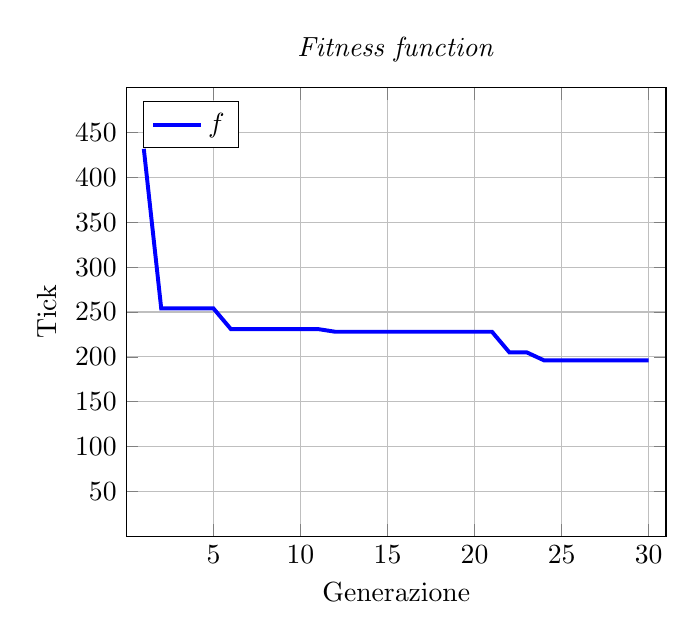
\begin{tikzpicture}
                \begin{axis}[
                    title={\textit{Fitness function}},
                    xlabel={Generazione},
                    ylabel={Tick},
                    xmin=0, xmax=31,
                    ymin=0, ymax=500,
                    xtick={5,10,15,20,25,30},
                    ytick={50, 100, 150, 200, 250, 300, 350, 400, 450},
                    legend pos=north west,
                    grid=major,
                    %ymajorgrids=true,
                    %xmajorgrids=true
                    %grid style=dashed,
                ]
                
                \addplot[
                    color=blue,
                    line width=0.5mm,
                    ]
                    coordinates {
                        (1,432.0)(2,254.0)(3,254.0)(4,254.0)(5,254.0)(6,231.0)(7,231.0)(8,231.0)(9,231.0)(10,231.0)(11,231.0)(12,228.0)(13,228.0)(14,228.0)(15,228.0)(16,228.0)(17,228.0)(18,228.0)(19,228.0)(20,228.0)(21,228.0)(22,205.0)(23,205.0)(24,196.0)(25,196.0)(26,196.0)(27,196.0)(28,196.0)(29,196.0)(30,196.0)
                    };
                    \legend{$f$}
                
                \end{axis}
            \end{tikzpicture}
        }
    \end{center}
    \caption{Andamento della funzione obiettivo al variare di generazione.}
    \label{modello3d_feromone}
\end{figure}   
    